\subsubsection{Design}
\subsubsection*{Architektur und Abhängigkeiten}
Bei der Wahl von Technologien, Tools und Frameworks achtete man besonders darauf, dass die entsprechenden Tools auch in der Zukunft noch supported werden. Dazu wurde geschaut, ob und wie gross die Community hinter einzelnen Tools ist und wie gut die Tools dokumentiert sind.

\subsubsection*{Applikations Architektur}
Für die Umsetzung der Anwendung hatte man zwei Optionen. Entweder man entwickelt eine Native App, also eine klassische Client-Server Anwendung, oder eine Web Anwendung. \\

Native Apps haben zwar einige Vorteile. Die Integration mit anderen Anwendungen ist so zum Beispiel einfacher. Zudem wäre die Monetarisierung auch um einiges einfacher, denn eine Native App kann sehr gut im App Store platziert werden. So steigt auch gleich die Bekanntheit der Applikation.\footcite{native_app} \\

Die Entscheidung bei der Entwicklung von Aufgaben-Coaching fiel jedoch sehr schnell auf eine Web Anwendung. Viele Schulen haben zwar Apple iPads im Einsatz. Trotzdem kann es Schulen geben, welche mit Android Tablets arbeiten. Da die Anwendung aber über den Browser läuft, muss nur eine Anwendung entwickelt werden. Bei einer Native App müsste man für Apple und Android je eine Anwendung entwickeln. Für grosse Firmen ist dies kein Problem, aber möchte man die Idee als Startup weiter verfolgen, hat man zu Beginn weder die Zeit noch das Kapital um gleich zwei Apps zu entwickeln. \\
Zudem kann man mit Web Anwendungen die Supportkosten relativ tief halten, was auf Schulen vielleicht noch ein bisschen attraktiver wirkt. Die Anwendung kann direkt im Browser aufgerufen werden und es muss nichts im vorhinein auf jedem Device installiert werden.

\begin{figure}[H]
\begin{center}
	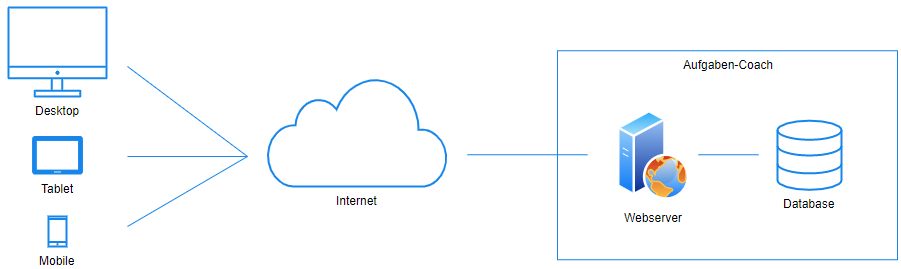
\includegraphics[width=\textwidth, keepaspectratio]{images/system_overview.png}
	\caption{System Overview}
	\label{fig:system_overview}
\end{center}
\end{figure}


\subsubsection*{Programmiersprache}
Für das Web Development gibt es mehrere Programmiersprachen, die zur Auswahl standen. Die Wohl bekanntesten darunter sind:

%https://en.wikipedia.org/wiki/Web_framework

\begin{itemize}
	\item Python (Django / Flask)
	\item C\# (ASP.NET Core)
	\item Java (Spring)
	\item JavaScript (Express.js / Node.js / Sails.js)
	\item PHP (CakePHP / CodeIgniter / Laravel)
	\item Perl (Catalyst / Mojolicious)
	\item Ruby (Ruby on Rails)
\end{itemize}

%TODO Satzstellung anschauen

Die Wahl fiel schnell auf Python, da bereits etwas KnowHow über diese Programmiersprache vorhanden ist. \\
Gemäss Developer Survey Results\footcite{developer_survey_results} von Stack Overflow ist Python (41.7\%) etwas bekannter als Java (41.1\%). Nur JavaScript (67.8\%) ist noch bekannter. In den letzten Jahren ist die Bekanntheit von Python auch noch weiter gestiegen. Man geht also davon aus, dass man auch in Zukunft noch mit Python arbeiten kann.


\subsubsection*{Web Framework}
Bei Python selber steht man vor der Auswahl von verschiedenen Web Frameworks. Gemäss einer Umfrage von JetBrains über Python wird die Frage ''What web frameworks / libraries do you use in addition to Python?'' mit dem Kommentar ''Django and Flask continue to be by far the most popular Python web frameworks.'' zusammen gefasst. \\
Laut der oben genannten Umfrage verwenden 43\% der Entwickler  Django als Web Framework. Flask folgt dicht darauf mit 41\%. Das nächst bekannteste Framework ist Tornado mit nur 6\%. \\
Bei der Evaluation konzentrierte man sich deshalb hauptsächlich auf Django und Flask. Mit bekannteren Frameworks hat man den Vorteil, dass es einfacher ist, Hilfe und gute Dokumentationen zu finden. Mit weit verbreiteten Technologien kann man auch davon ausgehen, dass diese noch längere Zeit bestehen bleiben.  \\ 

%TODO zitat einbauen
Flask\footcite{flask:foreword} beschreibt sich selber mit den Worten:

\begin{displayquote}
Flask is a lightweight WSGI web application framework. It is designed to make getting started quick and easy, with the ability to scale up to complex applications. It began as a simple wrapper around Werkzeug and Jinja and has become one of the most popular Python web application frameworks. \\
Flask offers suggestions, but doesn't enforce any dependencies or project layout. It is up to the developer to choose the tools and libraries they want to use. There are many extensions provided by the community that make adding new functionality easy.'
\end{displayquote}

Bei der Studienarbeit verwendete man bereits Flask zum Erstellen einer Webanwendung. Flask ist sicherlich ein gutes Framework, sonst würde es nicht von 41\% der Entwickler genutzt. Der grosse Vorteil von Flask ist, dass man als Entwickler relativ frei ist, wie man etwas umsetzen möchte. So kommt Flask standardmässig ohne Database Abstraction Layer, Form Validation oder anderen Tools, da bereits Libraries existieren, welche dies erledigen\footcite{flask:design}. Gerade am Anfang kann dies jedoch eher Verwirrung stiften, weil für das selbe Problem mehrere Lösungen bereit stehen. \\

Django verfolgt dagegen eher den Ansatz, bereits unterschiedliche Funktionalitäten mitzuliefern, was den Entwicklern Arbeit abnehmen soll. So ist zum Beispiel bereits ein OR-Mapper oder ein Admin Interface integriert\footcite{django:overview}. 
Django kommt aber auch mit einigen Nachteilen. Da einige Entscheidungen bereits vom Framework selber getroffen wurden, ist man als Entwickler nicht mehr ganz so flexibel. Zudem ist Django sehr monolithisch. Bei bestimmten Aufgaben ist vorgegeben, wie diese in Django umgesetzt werden müssen. Hält man sich nicht an den ''Django Way'', kann unter Umständen die gesamte Anwendung nicht deployed werden\footcite{django:advantages_disadvantages}.

In der Studienarbeit konnte man zwar bereits Erfahrung mit Flask sammeln, dennoch entschied man sich für Django. Besonders das Django als ''Fully Loaded Framework'' und mit einem integrierten Admin Interface daher kommt, wurde als sehr positiv erachtet.


\subsubsection*{Datenbank}
Um ein Datenbanksystem kommt diese Anwendung nicht herum. Folgende Überlegungen wurden sich bei der Evaluation für eine geeignete Datenbank gemacht:

\begin{itemize}
	\item Die Datenbank muss skalierbar sein, so dass sie auch eine grosse Anzahl Benutzer unterstützt.
	\item Da ein Grossteil der Benutzer mit Mobile Devices auf die Anwendung zugreift, soll bei Anfragen möglichst wenig Overhead geliefert werden.
	\item Die Schreib- und Lese-Operationen sind wichtig, jedoch nicht kritisch. 
\end{itemize}

Aufgrund der ohnehin schon verkürzten Projektlaufzeit entschied man sich, auf die Evaluation eines Datenbanksystems zu verzichten. Während den Modulen Datenbanksysteme 1 \& 2 konnte bereits sehr viel Erfahrungen mit Postgres gesammelt werden. Laut Deployment Statistics\footcite{deploymentstatistics} von Django Sites verwenden 47.7\% aller deployten Sites MySQL als Datenbank. Postgres folgt mit 40.7\%. Das nächst grössere Datenbanksystem ist sqlite mit nur noch 7.6\%.
MySQL wird zwar etwas öfters verwendet. Aus Erfahrung weiss man aber, dass die Funktionen von Postgres die Bedürfnisse dieser Anwendung voll und ganz abdecken, weshalb man Postgres als Datenbanksystem festlegte. \\

Sollte man in Zukunft jedoch ein anderes Datenbanksystem bevorzugen, kann die Migration mit dem Django Management Tool durchgeführt werden \footcite{dbmigration}. 

\subsubsection*{Python Libraries}

\subsubsection{UI Design}
Bevor mit der Entwicklung des Frontends begonnen werden kann, muss geplant werden, wie dieses aussehen soll. Um ein möglichst gutes Ergebnis zu erzielen, ist es wichtig sich folgende Fragen zu stellen:

\begin{itemize}
	\item Welche Anforderungen werden an die Webseite gestellt?
	\item Welche Benutzergruppen werden die Applikation verwenden?
	\item Was sind die Bedürfnisse der einzelnen Gruppen?
\end{itemize}

Durch das Beantworten der einzelnen Fragen, kann schnell herausgefunden werden, welche Anforderungen an das Frontend gestellt werden. Da der Aufgaben-Coach von komplett verschiedenen Benutzergruppen verwendet und damit gearbeitet wird, sollte das UI mögichst simpel und effizient gestaltet werden. Folgende Anforderungen konnten herauskristallisiert werden:

\begin{itemize}
	\item Usability \\
		Bei einer der Benutzergruppen handelt es sich um Schüler. Die Gruppe Schüler ist die Hauptnutzergruppe der Applikation und soll desshalb besonders gut abgeholt werden. Um möglichst auf ihre Bedürfnisse einzugehen, soll der komplette Teil, der für die Schüler gedacht ist, ebenfalls über Tablets und Mobiles bedienbar sein.
		
		%TODO https://www.jugendundmedien.ch/digitale-medien/fakten-zahlen.html
		
	\item Struktur \\
		Internetnutzer haben in der Regel eine relativ kurze Aufmerksamkeitsspanne, weshalb anhand der Struktur auf den ersten Blick klar sein sollte, was auf der Webseite möglich ist und was nicht. 
		
		%TODO https://www.websitebuilder-test.com/homepage-erstellen/#struktur
		
	\item Navigation \\
		Die Navigation über die Webseite soll so einfach und simpel wie möglich gehalten werden. Es soll möglich sein von jedem beliebigen Punkt der Webseite in kürzester Zeit zu einem beliebig anderen Punkt navigieren zu können.
		
		%TODO https://www.usability-tipps.de/info/index.php/erprobte-mittel-zur-wahrung-orientierung-webseiten/
	
	\item Orientierung \\
		Die Benutzer der Applikation sollen sich auf der Webseite zurecht finden und zu jedem Zeitpunkt wissen, wo sie sich befinden. Eine einfache Orientierung ist der Grundstein für das Wohlbefinden der Benutzer und soll deshalb berücksichtigt werden.
		
	\item Kontrast \\
		Die dargestellten Elemente sollen gut erkennbar sein und nicht in der Webseite versinken. Natürlich soll damit nicht übertrieben und mit knalligen Farben um sich geworfen werden.
\end{itemize}

Basierend auf den oben aufgelisteten UI-Design Anforderungen, wurden folgende Entscheidungen getroffen:

\begin{itemize}
	\item Usability \\
		Webseiten welche über Tablets und Mobilies verwendet werden, sollten niemals überladen sein. Aus diesem Grund sollen die Teile der Applikation, welche für die Schüler gedacht sind, schlicht und einfach gehalten werden. Wo auch immer möglich soll auf lange Texte verzichtet werden. Die einzelnen Seiten der Webapplikation sollen nur die für sie gedachte Aufgabe lösen.
		
		%TODO https://www.cubetech.ch/mobile-first-nur-ein-trend-oder-schon-bald-die-zukunft/
		
	\item Struktur \\
		Um eine möglichst benutzerfreundliche Struktur aufzubauen, soll auf ein Kompromiss zwischen, ''eine Webseite so einfach wie möglich halten und nur eine bestimmte Aufgabe lösen zu lassen'' und ''eine bestimmte Aufgabe mit so wenigen Klicks wie möglich lösen zu können'', gesetzt werden. \\
		
	\item Navigation \\
		Um eine schnelle Navigation zu ermöglichen, soll die Applikation in fünf Bereiche aufgeteilt werden, welche über die Navigationsleite erreichbar sind. Dabei soll es sich um folgende Bereiche handeln: Statistiken, Klassenverwaltung, Adminpanel, Schulstoff und User. 
		
	\item Orientierung \\
		Um den Benutzern eine möglichst gute Orientierung zu gewähren, sollen Breadcrumbs eingebaut werden. Um zusätzlich eine einheitliche Navigation durch die Applikation zu bieten, sollen die Breadcrumbs auch zum navigieren verwendet werden können.
		
	\item Kontrast \\
		Es soll auf knallige Farben und Eye­cat­cher verzichtet werden. Wichtige Elemente sollen zwar mit Farbe hervorgehoben werden, jedoch nicht dadurch auffallen. Die schlichte Gestalltung der Webseite soll die Aufmerksamkeit auf die entsprechenden Elemente leiten.
\end{itemize}


\subsubsection*{Mockup}
%TODO https://www.iqual.ch/de/internet-glossar/mockups
Anhand der getroffenen Entscheidungen wurden Mockups erstellt. Der Entscheid zum Erstellen von Mockups hat mehrere Gründe und bietet auch gleich verschiedene Vorteile. Während dem Erstellen von Mockups kann bereits früh erkannt werden, ob wichtige Punkte vergessen oder vernachlässigt wurden. Sobald die Mockups fertiggestellt sind, können damit bereits erste Tests durchgeführt werden. Zum Beispiel kann geprüft werden, ob alle geforderten funktionalen Anforderungen erfüllt werden und es können erstmals Usability-Tests durchgeführt werden, was viel Zeit und unnötige Arbeit ersparen kann. \\

Nachfolgend werden einige Beispiele für Ergebnisse der getroffenen Entscheidungen für die Mockups aufgelistet. Im Anhang sind alle gemachten Mockups zu finden. \\ %TODO Link zu Anhang einbauen.

Usability: \\
Auf dem Dashboard wird der Wochenplan des Schülers, gefolgt von den derzeit besuchten Fächern, knapp und ersichtlich aufgelistet. \\
\begin{minipage}{\textwidth}
	\begin{figure}[H]
	\centering
		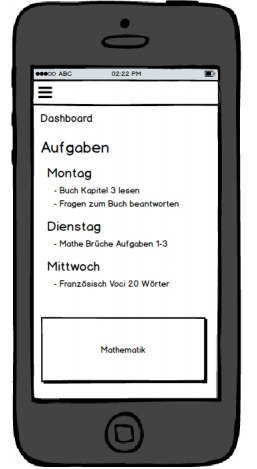
\includegraphics[width=5cm, keepaspectratio]{images/Mockups/Dashboard_Smartphone.png}
		\caption{Mockup Smartphone Dashboard}
	\end{figure}
\end{minipage}


Struktur: \\
Die Aufgabe dieser Seite ist es, neue Fragen zu definieren. Mit dem Risiko die Seite ein wenig zu überladen, dem Benutzer jedoch eine bessere Übersicht zu bieten, wurde ein Kompromiss eingegangen und entschieden, dass auch die dazugehörenden Hilfestellungen erfasst werden können. \\
\begin{minipage}{\textwidth}
	\begin{figure}[H]
	\centering
		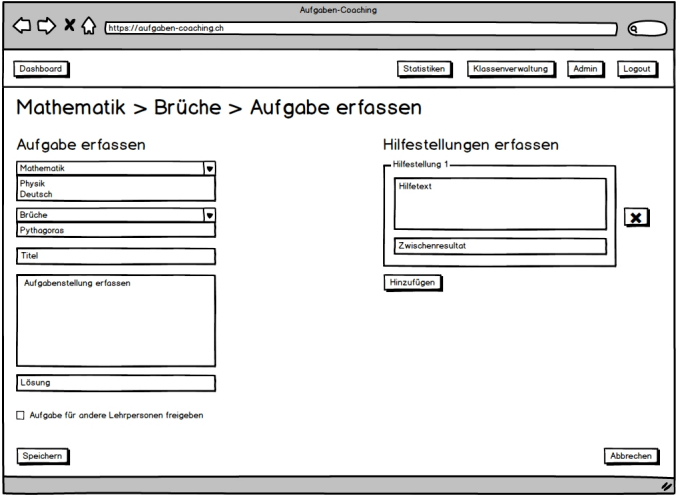
\includegraphics[width=\textwidth, keepaspectratio]{images/Mockups/AufgabeErfassen_Desktop.png}
		\caption{Mockup Aufgabe erfassen Desktop}
	\end{figure}
\end{minipage}


Navigation: \\
In der Navigationsbar sind die fünf definierten Bereiche ersichtlich. Dashboard stellt den Schulstoff Bereich dar, Statistiken die Statistiken, Klassenverwaltung die Klassenverwaltung, Admin das Adminpanel und Logout/Login die User. \\
\begin{minipage}{\textwidth}
	\begin{figure}[H]
	\centering
		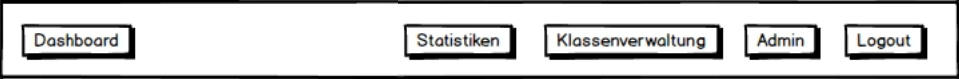
\includegraphics[width=\textwidth, keepaspectratio]{images/Mockups/Navigationsleiste_Desktop.png}
		\caption{Mockup Navigationsbar Desktop}
	\end{figure}
\end{minipage}


Orientierung: \\
Durch die Breadcrumbs wird hierarchisch dargestellt, wo man sich aktuell in der Webapplikation befindet. Mit einem Klick auf die übergeordneten Bereiche, navigiert man sofort an die gewünschte Stelle. \\
\begin{minipage}{\textwidth}
	\begin{figure}[H]
	\centering
		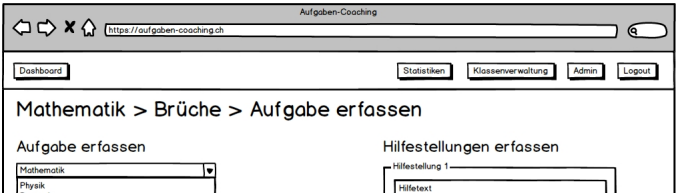
\includegraphics[width=\textwidth, keepaspectratio]{images/Mockups/Breadcrumbs_Desktop.png}
		\caption{Mockup Breadcrumbs Desktop}
	\end{figure}
\end{minipage}


Kontrast: \\
Da die Mockups in schwarz und weiss erstellt wurden, gibt es hierfür kein Beispiel. Die Entscheidung wurde natürlich dennoch in die Entwicklung miteinbezogen.



\subsubsection*{Effektive Webseite}

\newpage